% Version 1.2 of SN LaTeX, November 2022
%
% See section 11 of the User Manual for version history 
%
%%%%%%%%%%%%%%%%%%%%%%%%%%%%%%%%%%%%%%%%%%%%%%%%%%%%%%%%%%%%%%%%%%%%%%
%%                                                                 %%
%% Please do not use \input{...} to include other tex files.       %%
%% Submit your LaTeX manuscript as one .tex document.              %%
%%                                                                 %%
%% All additional figures and files should be attached             %%
%% separately and not embedded in the \TeX\ document itself.       %%
%%                                                                 %%
%%%%%%%%%%%%%%%%%%%%%%%%%%%%%%%%%%%%%%%%%%%%%%%%%%%%%%%%%%%%%%%%%%%%%

%%\documentclass[referee,sn-basic]{sn-jnl}% referee option is meant for double line spacing

%%=======================================================%%
%% to print line numbers in the margin use lineno option %%
%%=======================================================%%

%%\documentclass[lineno,sn-basic]{sn-jnl}% Basic Springer Nature Reference Style/Chemistry Reference Style

%%======================================================%%
%% to compile with pdflatex/xelatex use pdflatex option %%
%%======================================================%%

%%\documentclass[pdflatex,sn-basic]{sn-jnl}% Basic Springer Nature Reference Style/Chemistry Reference Style


%%Note: the following reference styles support Namedate and Numbered referencing. By default the style follows the most common style. To switch between the options you can add or remove “Numbered” in the optional parenthesis. 
%%The option is available for: sn-basic.bst, sn-vancouver.bst, sn-chicago.bst, sn-mathphys.bst. %  
 
%%\documentclass[sn-nature]{sn-jnl}% Style for submissions to Nature Portfolio journals
%%\documentclass[sn-basic]{sn-jnl}% Basic Springer Nature Reference Style/Chemistry Reference Style
\documentclass[sn-mathphys,Numbered]{sn-jnl}% Math and Physical Sciences Reference Style
%%\documentclass[sn-aps]{sn-jnl}% American Physical Society (APS) Reference Style
%%\documentclass[sn-vancouver,Numbered]{sn-jnl}% Vancouver Reference Style
%%\documentclass[sn-apa]{sn-jnl}% APA Reference Style 
%%\documentclass[sn-chicago]{sn-jnl}% Chicago-based Humanities Reference Style
%%\documentclass[default]{sn-jnl}% Default
%%\documentclass[default,iicol]{sn-jnl}% Default with double column layout

%%%% Standard Packages
%%<additional latex packages if required can be included here>

\usepackage{graphicx}%
\usepackage{multirow}%
\usepackage{amsmath,amssymb,amsfonts}%
\usepackage{amsthm}%
\usepackage{mathrsfs}%
\usepackage[title]{appendix}%
\usepackage{xcolor}%
\usepackage{textcomp}%
\usepackage{manyfoot}%
\usepackage{booktabs}%
\usepackage{algorithm}%
\usepackage{algorithmicx}%
\usepackage{algpseudocode}%
\usepackage{listings}%
%%%%

%%%%%=============================================================================%%%%
%%%%  Remarks: This template is provided to aid authors with the preparation
%%%%  of original research articles intended for submission to journals published 
%%%%  by Springer Nature. The guidance has been prepared in partnership with 
%%%%  production teams to conform to Springer Nature technical requirements. 
%%%%  Editorial and presentation requirements differ among journal portfolios and 
%%%%  research disciplines. You may find sections in this template are irrelevant 
%%%%  to your work and are empowered to omit any such section if allowed by the 
%%%%  journal you intend to submit to. The submission guidelines and policies 
%%%%  of the journal take precedence. A detailed User Manual is available in the 
%%%%  template package for technical guidance.
%%%%%=============================================================================%%%%

%\jyear{2021}%
\raggedbottom
%%\unnumbered% uncomment this for unnumbered level heads

\begin{document}

\title[Article Title]{Supplementary Material for ``Developing Comprehensive Annotation Guidelines and a Corpus of Risk of Bias Assessment for Rehabilitation: A Methodological Approach''}

%%\pacs[JEL Classification]{D8, H51}

%%\pacs[MSC Classification]{35A01, 65L10, 65L12, 65L20, 65L70}

\maketitle


%%%%%%%%%%%%%%%%
%% Background %%
\section*{Annotation Guidelines}
\label{sec:guidelines}
%
In each of the following subsections, we describe the annotation guidelines for the signalling questions using the instructional placards developed through consultation with RoB assessment and natural language processing experts.

Each placard is a flowchart encoding instructions to guide annotators in annotating the RoB question by question for the signalling questions in the Revised Cochrane RoB tool 2.0.
The flowchart starts with the title informing the annotators of which question they are annotating for.
The first diamond in the actual instructional flowchart asks the annotators to look for specific information or part of the text and, if found, instructs them to annotate it.
There are little colour-coded arrows flanking the diamond instructing the annotators to first look for the information in the green arrow region (for e.g., in the Results section). 
If the information is not found in the green-coded arrow, check for it in the yellow-coded arrow (e.g., a table or a flowchart).
If for a particular question, no information is found, we assume that the text did not have any information for that particular signalling question.
\textcolor{red}{Include a generic description about the colours, logos, shapes and flowchart elements in the placards here...}
%
%
%
\subsection*{Signalling question: 1.1}
%
OXO
%
%
%
\subsection*{Signalling question: 1.2}
%
OXO
%
%
%
\subsection*{Signalling question: 1.3}
%
OXO
%
%
%
\subsection*{Signalling question - 2.3}
\label{subsec:2_3}
%
For annotation instructions for this signalling question, ``Were there deviations from the intended intervention that arose because of the trial context?'' follow the Flowchart~\ref{fig:2_3}.
%
\begin{figure}[hbt]
    \centering
    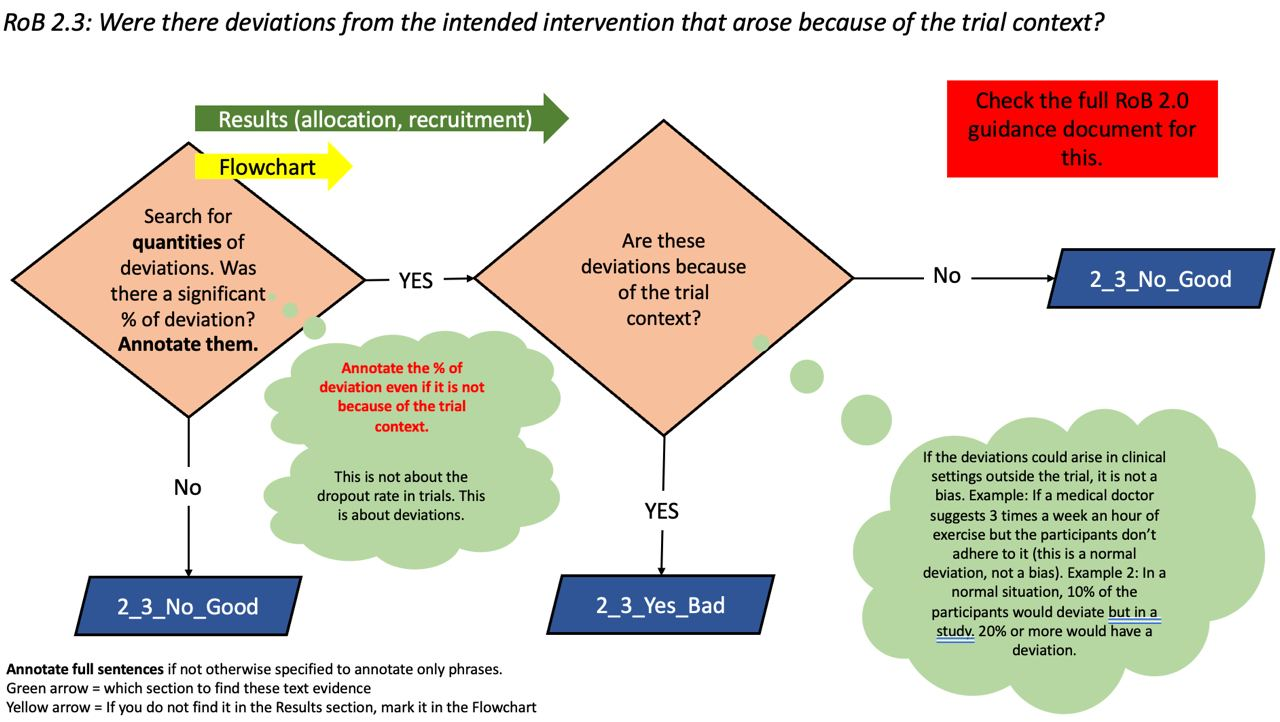
\includegraphics[width=\textwidth]{figures/2_3.jpg}
    \caption{Annotation instructions for the RoB 2.3 signalling question.}
    \label{fig:2_3}
\end{figure}
%
The first diamond in the flowchart asks the annotators to search for quantities of deviation with a thought bubble hinting to them that these deviations are not the dropout rate in the trial.
Deviations from the intended intervention are defined as any unintentional changes that may have occurred in the intervention being studied due to the trial context. 
For example, participants may not have complied with the study protocol, or there may have been problems with the delivery of the intervention that could have influenced the study outcomes.
Dropouts, on the other hand, refer to participants who withdrew from the study or were lost to follow-up.
Dropout rates can potentially introduce bias into a study if the characteristics of the participants who dropped out are different from those who completed the study.
High dropout rates can also affect the statistical power of the study and its ability to draw valid conclusions.
While both deviations from the intended intervention and dropout rates can potentially introduce bias into a study, they are not the same thing and should be evaluated separately when assessing the risk of bias in a study.
The diamond element also hints to the annotators that they can find this information in the text of the Results section, either within the allocation paragraph or the recruitment paragraph (green-coded arrow).
If the information was not found within the Results section, look for it in the flowchart (either the flowcharts themselves or their captions).
If no percentage or deviation or the number of deviations were identified in the text, do not annotate anything, and this document will be automatically marked as a ``No information'' for this signalling question.
If the percentage of deviation was identified, then annotate the full sentence where this information is found.
Next, go to the next diamond following the ``yes'' flow and judge whether these deviations were due to the trial context.
If the deviations arose due to trial context, mark the annotated text as ``2.3 Yes Bad'' and ``2.3 No Good'' otherwise.
Now this part is quite subjective, but at least we have the annotated information about the percentage/number of deviations which could be used to train the ML models.
We let the reviewers be a judge of the trial context once they discover the deviation information.
Ultimately, the review of deviations and trial context is subjective, but the annotated information can be used to train machine learning models.
%
%
%
\subsection*{Signalling question - 2.4 }
%
For annotation instructions for this signalling question, ``Were these deviations likely to have affected the outcome?'' follow the Flowchart~\ref{fig:2_4}.
%
\begin{figure}[hbt]
    \centering
    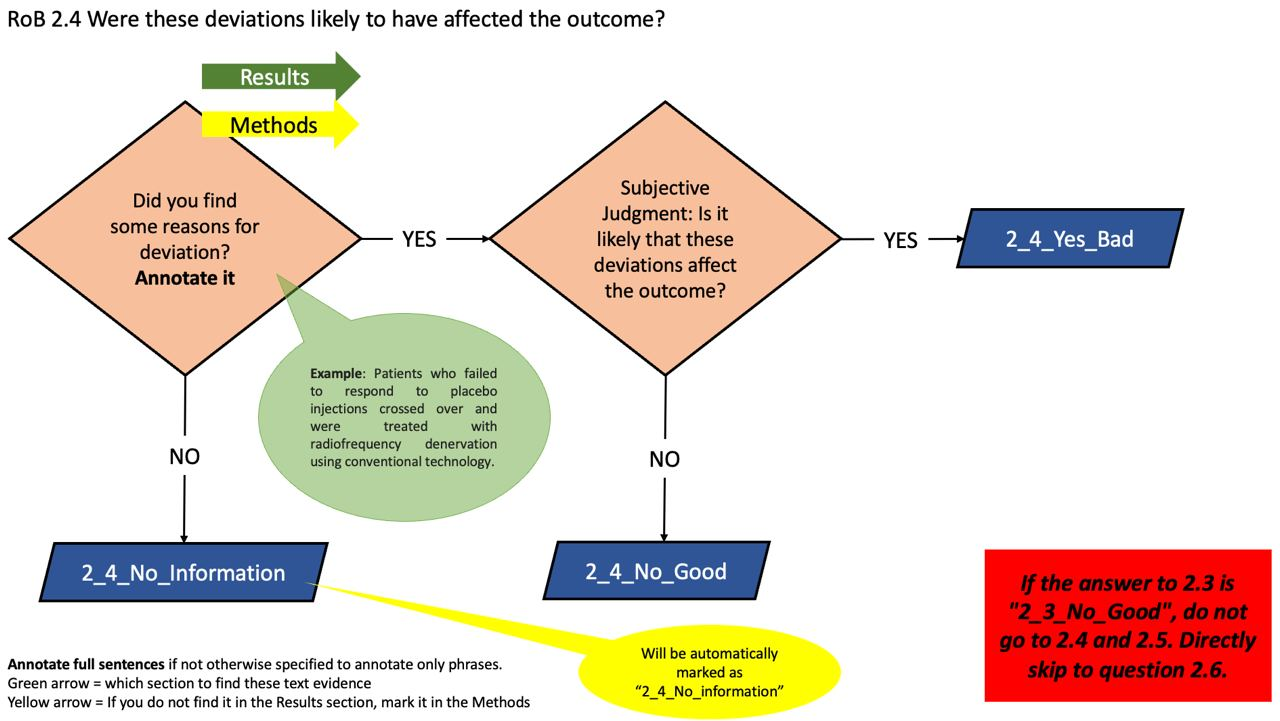
\includegraphics[width=\textwidth]{figures/2_4.jpg}
    \caption{Annotation instructions for the RoB 2.4 signalling question.}
    \label{fig:2_4}
\end{figure}
%
Do not annotate for this question if the answer to the previous question was ``2.3 No Good'' otherwise, follow the instructions below.
In randomized clinical trials, deviations from the planned study protocol may occur for various reasons, such as the participant not following the intervention as intended or the trial site not adhering to the study procedures.
These deviations are known as "protocol deviations" or "protocol violations."
The question "Were these deviations likely to have affected the outcome?" in the revised Cochrane RoB 2.0 tool refers to whether the protocol deviations had the potential to influence the study results.
The aim of this question is to assess the RoB due to the protocol deviations, which may have introduced systematic error or affected the internal validity of the study.
If the deviations were unlikely to have affected the study outcome, then this question would be answered with "No."
However, if the deviations were likely to have affected the study outcome, then this question would be answered with "Yes," indicating that the study is at high risk of bias.
If it is unclear whether the deviations affected the outcome, the answer would be "Some concerns."
To annotate the information from the previous question, we identify the percentage of deviation (a number) and annotate it, while for this question we look for the reasons for these deviations and annotate them.
The reasons could be found in either the Results section or in the Method section if not in the Results section.
If you identify the reason for this deviation and mark it then follow the path along ``yes'' and judge whether these deviations could affect the outcome.
If they do, mark the annotated reason for deviation as ``2.4 Yes Bad'' and ``2.4 No Good''otherwise.
%
%
%
\subsection*{Signalling question - 2.5 }
%
For annotation instructions for this signalling question, ``Were these deviations from the intended intervention balanced between groups??'' follow the Flowchart~\ref{fig:2_5}.
%
\begin{figure}[hbt]
    \centering
    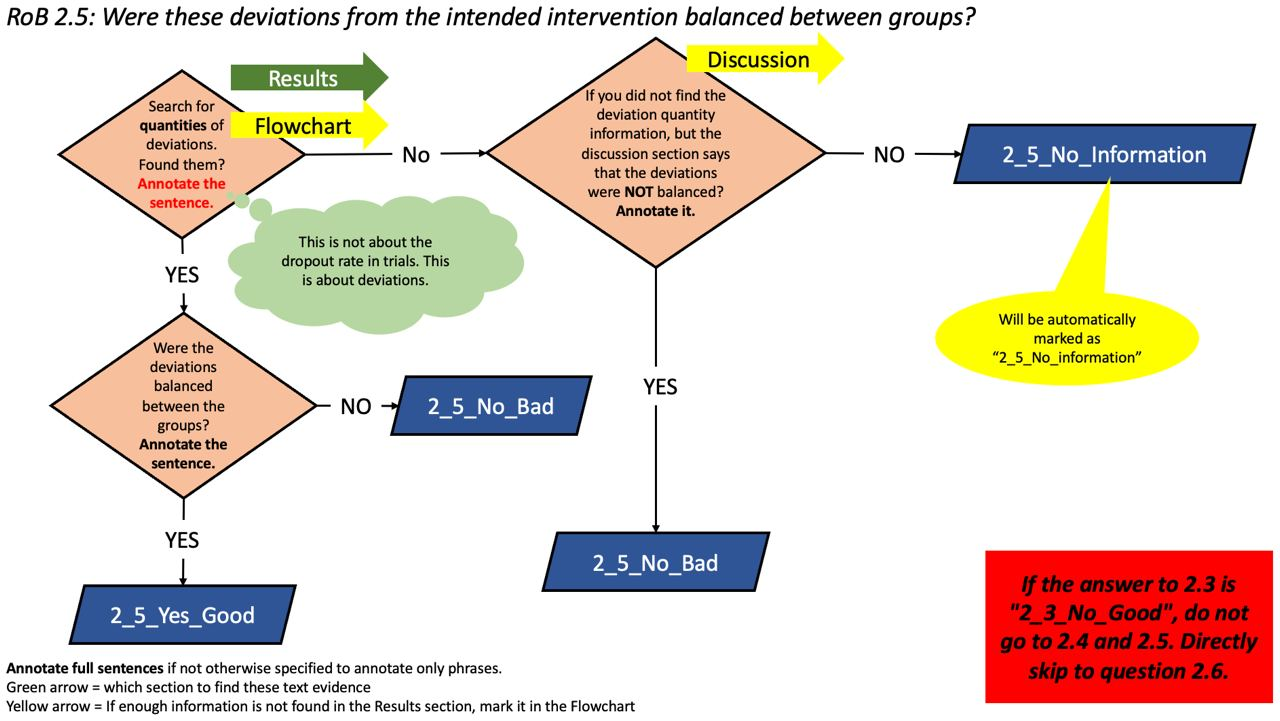
\includegraphics[width=\textwidth]{figures/2_5.jpg}
    \caption{Annotation instructions for the RoB 2.5 signalling question.}
    \label{fig:2_5}
\end{figure}
%
In the context of a randomized controlled trial (RCT), the intended intervention refers to the intervention that was supposed to be given to the study participants according to the study protocol. However, sometimes deviations from the intended intervention may occur due to various reasons, such as participant non-compliance or study staff error.

The question "Were these deviations from the intended intervention balanced between groups?" is asking whether any deviations from the intended intervention were similar in frequency and severity across the different study groups (i.e., intervention group and control group) or whether one group had a greater number or severity of deviations than the other.

Balanced deviations between groups are important for maintaining the internal validity of the study. If one group had a higher number or severity of deviations from the intended intervention than the other, it could potentially introduce bias and confound the results of the study. Therefore, it is important to assess whether deviations from the intended intervention were balanced between the groups when evaluating the risk of bias in an RCT.

The first diamond in the flowchart asks the annotators to search for quantities of deviation with a thought bubble hinting to them that these deviations are not the dropout rate in the trial (to understand the difference between deviations and dropout, refer to subsection~\ref{subsec:2_3}).
If the deviations were balanced between the groups, mark the annotated deviations as ``2.5 Yes Good'' and ``2.5 No Bad'' otherwise.
Now if you did not find any quantification of the deviations but found the text in the Discussion section saying that the deviations were not balanced, then mark such text in the discussion as ``2.5 No Bad''.
%
%
%
%
\subsection*{Signalling question - 2.7 }
%
For annotation instructions for this signalling question, ``Was there potential for a substantial impact (on the result) of the failure to analyse participants in the group to which they were randomized?'' follow the Flowchart~\ref{fig:2_7}.
%
\begin{figure}[hbt]
    \centering
    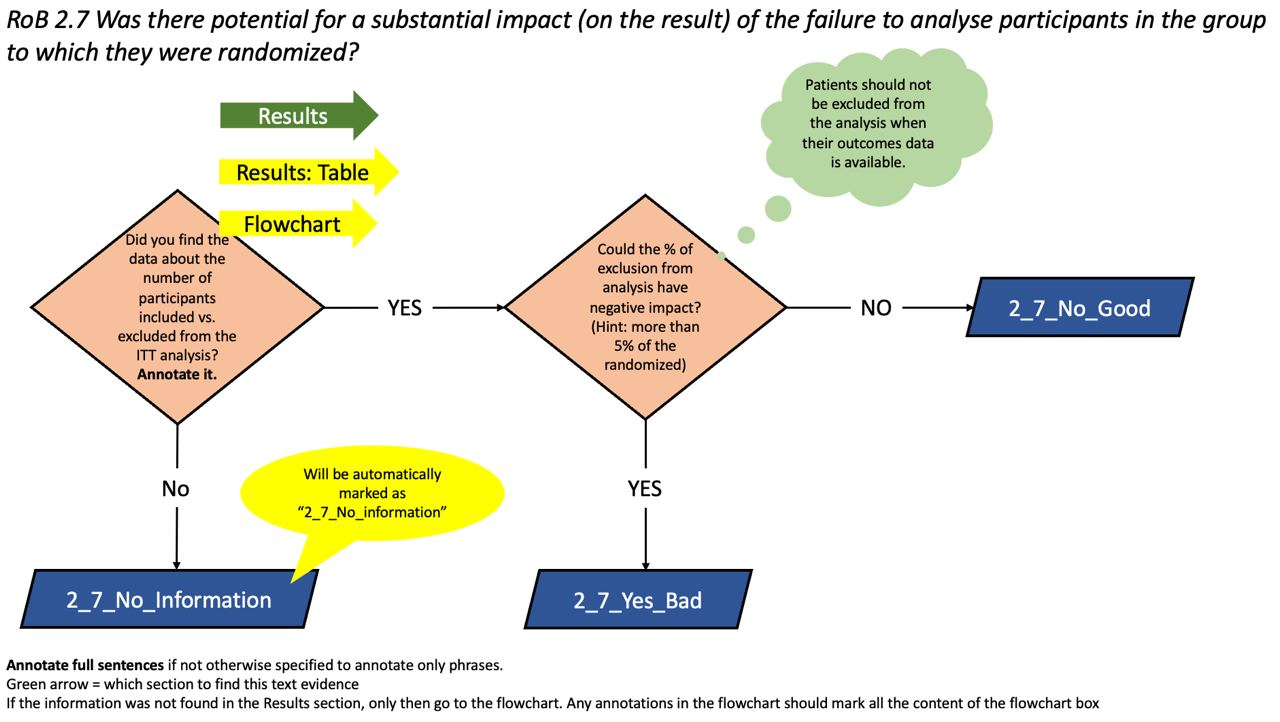
\includegraphics[width=\textwidth]{figures/2_7.jpg}
    \caption{Annotation instructions for the RoB 2.7 signalling question.}
    \label{fig:2_7}
\end{figure}


The question ``Was there potential for a substantial impact (on the result) of the failure to analyze participants in the group to which they were randomized?'' in the Cochrane Risk of Bias (RoB) 2.0 tool refers to the risk of bias associated with deviations from the intended analysis plan in a randomized controlled trial (RCT).

In an RCT, participants are usually randomized to receive either the intervention being tested or a control intervention. The analysis plan is typically based on the assumption that all participants will be analyzed according to the group to which they were randomized. However, there may be instances where participants are not analyzed in the group to which they were randomized, for example, if they dropped out of the study or if they switched groups. This is known as a deviation from the intended analysis plan.

The question is asking whether this deviation from the intended analysis plan could have had a substantial impact on the study results. If there is a potential for a substantial impact, then there is a high risk of bias. For example, if a large proportion of participants in the intervention group dropped out of the study, but all participants in the control group were analyzed, this could lead to an overestimation of the treatment effect. Similarly, if participants switched groups, this could lead to an underestimation or overestimation of the treatment effect.

Therefore, this question is important for assessing the risk of bias associated with deviations from the intended analysis plan in an RCT, and it helps to ensure that the study results are reliable and valid.


The analysis we focus on this question is ITT or intent-to-treat analysis.
The first diamond asks the annotators to find the number of people included in the ITT analysis vs. the number of people randomized to each of the intervention/comparator groups. 
If this information is found, annotate it and follow the ``yes'' flow in the diagram.
Now examine whether the percentage of participants excluded from the ITT analysis could have had a negative impact.
We also include a hint here, and if more than 5\% of randomized participants were excluded from ITT analysis, we ask the annotators to mark the text as ``2.7 Yes Bad'' and ``2.7 No Good'' otherwise.
%
%
%
%%===========================================================================================%%
%% If you are submitting to one of the Nature Portfolio journals using the eJP submission   %%
%% system, please include the references within the manuscript file itself. You may do this  %%
%% by copying the reference list from your .bbl file, paste it into the main manuscript .tex %%
%% file, and delete the associated \verb+\bibliography+ commands.                            %%
%%===========================================================================================%%

\bibliography{sn-bibliography.bib}% common bib file
%% if required, the content of the .bbl file can be included here once bbl is generated
%%\input sn-article.bbl


\end{document}
